% !TeX encoding = UTF-8
% Use XeLaTeX to compile it

\documentclass[a4paper,12pt]{book}

\RequirePackage{polyglossia}
 \setdefaultlanguage{russian}
 \setotherlanguage{english}

\RequirePackage{fontspec}
 \setmainfont{CMU Serif}
 \setsansfont{CMU Sans Serif}
 \setmonofont{CMU Typewriter Text}

\RequirePackage{hyperref}
\hypersetup{
	colorlinks
}

\RequirePackage[usenames,dvipsnames]{xcolor}
\RequirePackage{graphicx}
\RequirePackage{wrapfig}
\RequirePackage{textpos}
\RequirePackage{perpage}
\MakePerPage{footnote}

\RequirePackage{geometry}
\geometry{
	a4paper,
	left=35mm,
	right=25mm,
	top=30mm,
	bottom=30mm,
}

\renewcommand{\baselinestretch}{1.15}
\newcommand*{\btw}[1]{\vspace{10pt}\emph{#1}\vspace{10pt}}
\newcommand*{\note}[1]{\vspace{10pt}
\textcolor{Mahogany}{\textbf{\large#1}}
\vspace{10pt}
}
\newcommand{\code}[1]{\verb|#1|}

\title{Snake Wrangling for Kids - Learning to Program with Python}
\author{Jason R Briggs}

\makeindex

\begin{document}
\pagestyle{empty}
\frontmatter
\begin{FRONTCOVER}
\begin{titlepage}
\begin{textblock*}{210mm}(0mm,0mm)
   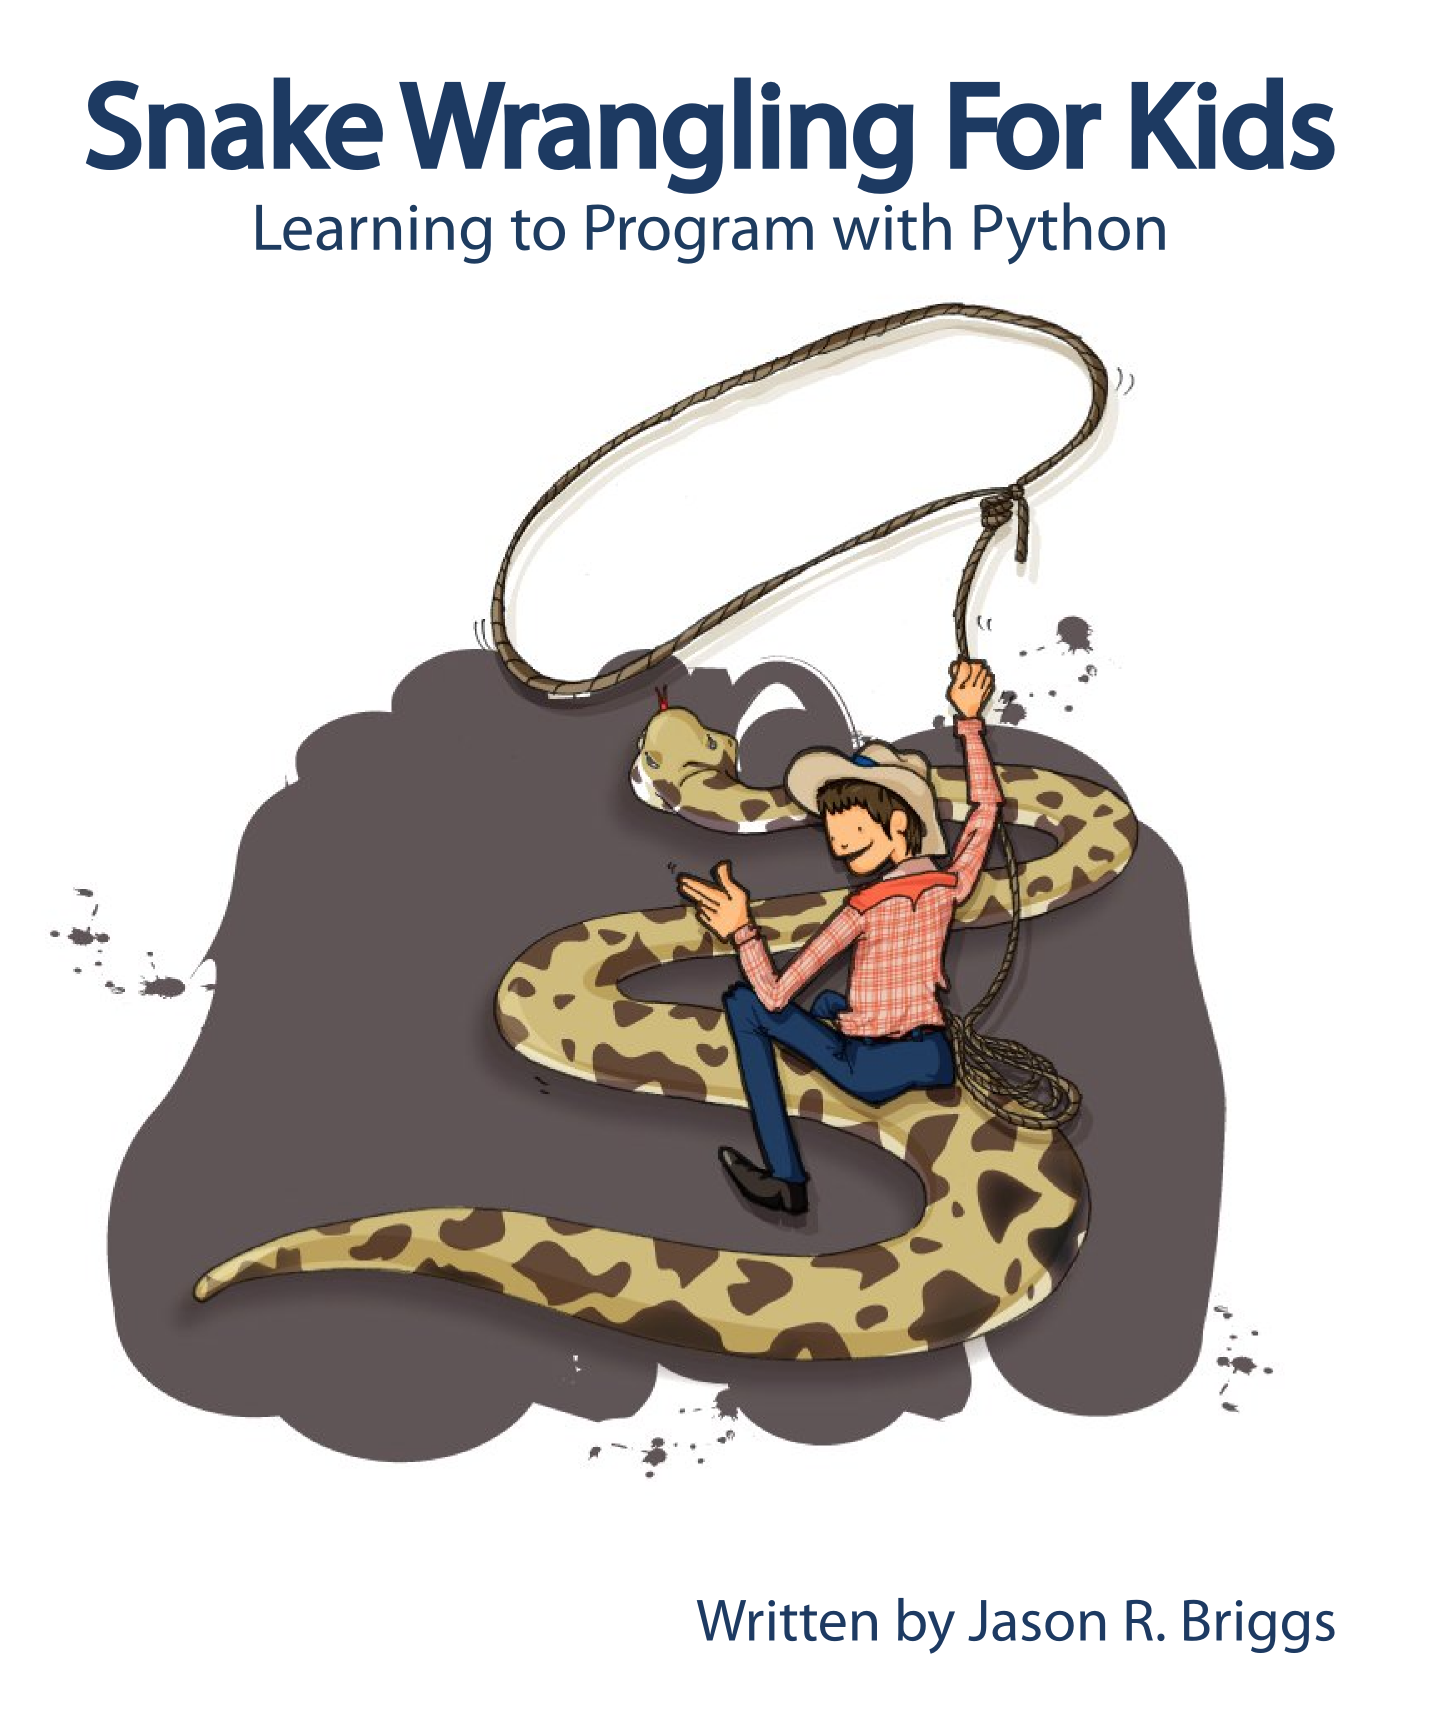
\includegraphics[width=0.9\paperwidth]{cover.eps}
\end{textblock*}
\begin{flushright}
\begin{WINDOWS}
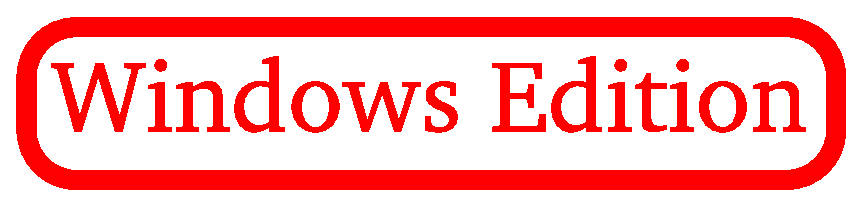
\includegraphics[width=40mm]{windows-edition.eps} 
\end{WINDOWS}
\begin{MAC}
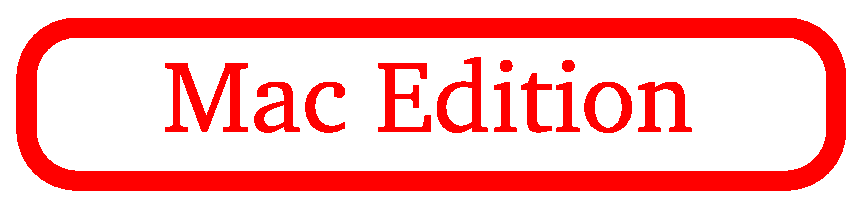
\includegraphics[width=40mm]{mac-edition.eps} 
\end{MAC}
\begin{LINUX}

\includegraphics[width=40mm]{linux-edition.eps} 
\end{LINUX}
\end{flushright}
\end{titlepage}
\end{FRONTCOVER}

\noindent
\textsf{\emph{Snake Wrangling for Kids, Learning to Program with Python}}\\
by Jason R. Briggs\\
\\
Version 0.7.7
\\\\
Copyright \copyright 2007.\\
\\
Cover art and illustrations by Nuthapitol C.\\
\\
\noindent
\textsf{\emph{This book has been completely rewritten and updated, with new chapters (including developing graphical games), and new code examples. It also includes lots of fun programming puzzles to help cement the learning. Published by No Starch Press - available here: \href{http://nostarch.com/pythonforkids}{Python for Kids}. Also find more info \href{http://jasonrbriggs.com/python-for-kids/}{here}.}}
\\
\\
\linebreak
\noindent
Website:\\ \href{http://www.briggs.net.nz/log/writing/snake-wrangling-for-kids}{http://www.briggs.net.nz/log/writing/snake-wrangling-for-kids}\\ 
\\
\noindent
Thanks To:\\
Guido van Rossum (for benevelont dictatorship of the Python language), the members of the \href{http://www.python.org/community/sigs/current/edu-sig/}{Edu-Sig} mailing list (for helpful advice and commentary), author \href{http://www.davidbrin.com/}{David Brin} (the original \href{http://www.salon.com/tech/feature/2006/09/14/basic/}{instigator} of this book), Michel Weinachter (for providing better quality versions of the illustrations), and various people for providing feedback and errata, including: Paulo J. S. Silva, Tom Pohl, Janet Lathan, Martin Schimmels, and Mike Cariaso (among others).  Anyone left off this list, who shouldn't have been, is entirely due to premature senility on the part of the author.\\

\noindent
License:\\
\\
\includegraphics[width=40mm]{by-nc-sa.eps}\\
This work is licensed under the Creative Commons Attribution-Noncommercial-Share Alike 3.0 New Zealand License. To view a copy of this license, visit\\ \href{http://creativecommons.org/licenses/by-nc-sa/3.0/nz/}{http://creativecommons.org/licenses/by-nc-sa/3.0/nz/} or send a letter to Creative Commons, 171 Second Street, Suite 300, San Francisco, California, 94105, USA.\\

\noindent
Below is a summary of the license.\\

\noindent
You are free:
\begin{itemize}
 \item \textbf{to Share} — to copy, distribute and transmit the work 
 \item \textbf{to Remix} — to adapt the work
\end{itemize}
\noindent
Under the following conditions:
\begin{description}
 \item[Attribution.] You must attribute the work in the manner specified by the author or licensor (but not in any way that suggests that they endorse you or your use of the work).
 \item[Noncommercial.] You may not use this work for commercial purposes.
 \item[Share Alike.] If you alter, transform, or build upon this work, you may distribute the resulting work only under the same or similar license to this one.
\end{description}

\noindent
For any reuse or distribution, you must make clear to others the license terms of this work.\\

\noindent
Any of the above conditions can be waived if you get permission from the copyright holder.\\

\noindent
Nothing in this license impairs or restricts the author's moral rights.\\

\vspace*{4cm}
\begin{center}

\includegraphics[width=5cm]{python-powered.eps}
\end{center}

\mainmatter

\pagestyle{plain}

\pagenumbering{roman}
\tableofcontents
% preface.tex
% This work is licensed under the Creative Commons Attribution-Noncommercial-Share Alike 3.0 New Zealand License.
% To view a copy of this license, visit http://creativecommons.org/licenses/by-nc-sa/3.0/nz
% or send a letter to Creative Commons, 171 Second Street, Suite 300, San Francisco, California, 94105, USA.


\chapter*{Preface}\normalsize
    \addcontentsline{toc}{chapter}{Preface}
\begin{center}
{\em A Note to Parents...}
\end{center}
\pagestyle{plain}

\noindent
Dear Parental Unit or other Caregiver,

In order for your child to get started with programming, you're going to need to install Python on your computer.  This book has recently been updated to use Python 3.0--this latest version of Python is not compatible with earlier versions, so if you have an earlier version of Python installed, then you'll need to download an older release of the book.

Installing Python is a fairly straight-forward task, but there are a few wrinkles depending upon what sort of Operating System you're using.  If you've just bought a shiny new computer, have no idea what to do with it, and that previous statement has filled you with a severe case of the cold chills, you'll probably want to find someone to do this for you.  Depending upon the state of your computer, and the speed of your internet connection, this could take anything from 15 minutes to a few hours.

\begin{WINDOWS}

\noindent
First of all, go to \href{http://www.python.org}{www.python.org} and download the latest Windows installer for Python 3.  At time of writing, this is:
\begin{quote}
     \href{http://www.python.org/ftp/python/3.0/python-3.0.msi}{http://www.python.org/ftp/python/3.0/python-3.0.msi}
\end{quote}
Double-click the icon for the Windows installer (you do remember where you downloaded it to, don't you?), and then follow the instructions to install it in the default location (this is probably \emph{c:$\backslash$Python30} or something very similar).

\end{WINDOWS}

\begin{MAC}

\noindent
At time of writing, installing Python 3 on your Mac is a more complicated process than usual.  At the moment, there are no one-click install packages available.  There is information out there describing the installation process (here is a good \href{http://farmdev.com/thoughts/66/python-3-0-on-mac-os-x-alongside-2-6-2-5-etc-/}{page}), but the basic process is to download the source package and then build it yourself.  This isn't as difficult as it sounds, but you will need to follow a few steps in the Terminal.  If you find this too complicated, I recommend sticking with the \href{http://www.briggs.net.nz/log/wp-content/uploads/2008/03/swfk-mac.zip}{previous version} of this book.

\noindent
First of all, go to \href{www.python.org}{www.python.org} and download the Python source package. As of Dec 2008, the address for this download is:

\noindent
\href{http://www.python.org/ftp/python/3.0/Python-3.0.tar.bz2}{http://www.python.org/ftp/python/3.0/Python-3.0.tar.bz2}

\noindent
Start the Terminal application, and enter the following commands:

\begin{listing}
\begin{verbatim}
$ cd ~/Downloads/Python-3.0/
$ ./configure --enable-framework MACOSX_DEPLOYMENT_TARGET=10.5 --with-universal-archs=all
$ make && make test
$ sudo make frameworkinstall
\end{verbatim}
\end{listing}

\noindent
The following steps may, or may not, be necessary.  First of all type: 

\code{ls -la /Library/Frameworks/Python.framework/Versions/}

\noindent
In my case, there are only two directories shown:

\begin{listing}
\begin{verbatim}
    drwxr-xr-x  4 root  admin  136  6 Dec 23:31 .
    drwxr-xr-x  6 root  admin  204  6 Dec 23:31 ..
    drwxr-xr-x  9 root  admin  306  6 Dec 23:32 3.0
    lrwxr-xr-x  1 root  admin    3  6 Dec 23:31 Current -> 3.0
\end{verbatim}
\end{listing}

\noindent
If you have more than those two directories listed (for example)$\ldots$

\begin{listing}
\begin{verbatim}
    drwxr-xr-x  4 root  admin  136   6 Dec 23:31 .
    drwxr-xr-x  6 root  admin  204   6 Dec 23:31 ..
    drwxr-xr-x  9 root  admin  306   7 Nov 08:19 2.4
    drwxr-xr-x  9 root  admin  306  22 Mar 23:32 2.5
    drwxr-xr-x  9 root  admin  306  12 Dec 10:22 2.6
    drwxr-xr-x  9 root  admin  306   6 Dec 23:31 3.0
    lrwxr-xr-x  1 root  admin    3   6 Dec 23:31 Current -> 3.0
\end{verbatim}
\end{listing}

\noindent
$\ldots$then you may need to perform the following steps:

\begin{listing}
\begin{verbatim}
$ cd /Library/Frameworks/Python.framework/Versions/
$ sudo rm Current
$ sudo ln -s 2.5 Current
\end{verbatim}
\end{listing}

Finally, you'll want to setup Python 3 as the default, for when your child opens the Terminal application. To do this you'll need to edit the path used by Terminal--start Terminal, and then enter the following command \code{pico ~/.bash\_profile}.  This file may (or may not) exist already, and if it does, there may (or may not) already be a path set up.  In any case, at the bottom of the file, add the following:

\begin{listing}
\begin{verbatim}
export PATH="/Library/Frameworks/Python.framework/Versions/3.0/bin:${PATH}"
\end{verbatim}
\end{listing}

Save your changes, by hitting CTRL+X, and typing Y to save. If you restart the Terminal app, and type \code{python}, with any luck, you should see something similar to the following:

\begin{listing}
\begin{verbatim}
Python 3.0 (r30:67503, Dec  6 2008, 23:22:48) 
[GCC 4.0.1 (Apple Inc. build 5465)] on darwin
Type "help", "copyright", "credits" or "license" for more information.
>>>
\end{verbatim}
\end{listing}

\end{MAC}

\begin{LINUX}

\noindent
First of all, download and install the latest version of Python 3 for your distribution.  Given the large number of Linux flavours, it's impossible to give exact details on installation for each---but chances are, if you're running Linux, you already know what you're doing anyway.  In fact, you're probably insulted by the very idea of being told how to install$\ldots$anything

\end{LINUX}

\noindent
\emph{\color{BrickRed}After installation$\ldots$}

\noindent
$\ldots$You might need to sit down next to your child for the first few chapters, but hopefully after a few examples, they should be batting your hands away from the keyboard to do it themselves.  They should, at least, know how to use a text editor of some kind before they start (no, not a Word Processor, like Microsoft Word---a plain, old-fashioned text editor)---they should at least able to open and close files, create new text files and save what they're doing.  Apart from that, this book will try to teach the basics from there.
\\
\\
\noindent\\
Thanks for your time, and kind regards,
\noindent\\
THE BOOK
% !TeX encoding = UTF-8
% Use XeLaTeX to compile it
%
% Эта работа распространяется на условиях лицензии Creative Commons Attribution-Noncommercial-Share Alike 3.0 New Zealand License.
% Краткое описание лицензии есть тут: http://creativecommons.org/licenses/by-nc-sa/3.0/nz/deed.ru
% Полное — там же.
% Эту книгу можно невозбранно распространять и изменять, но только соблюдая следующие условия:
% сохраняя лицензию и не вводя дополнительных ограничений, бесплатно
% и указывая авторство как оригинальной части, так и изменённой.
% Автор оригинального английского текста — Jason R Briggs http://jasonrbriggs.com/
% Автор перевода — Егор Кочетов <Egor.Kochetoff@gmail.com>
%
% This work is licensed under the Creative Commons Attribution-Noncommercial-Share Alike 3.0 New Zealand License.
% To view a copy of this license, visit http://creativecommons.org/licenses/by-nc-sa/3.0/nz
% or send a letter to Creative Commons, 171 Second Street, Suite 300, San Francisco, California, 94105, USA.
%

\chapter{Не все змеи будут шипеть на тебя}\label{ch:notallsnakeswillsquishyou}

Возможно, тебе подарили эту книгу на день рожденья. А может, на рождество. Например, так: тётя Агата (у всех есть тётя Агата, но не все об этом знают) хотела подарить носки, хотя и не парные, но оба красивые, на два размера больше — на вырост (и всё равно бы эти носки не пригодились потом). А потом вместо этого услышала про эту книгу (которую можно взять и напечатать), вспомнила твои вопросы про всякие компьютерные штуки, и твои непонятные объяснения, как пользоваться компьютером, оборвавшиеся в момент, когда она начала разговаривать с компьютерной мышью, и решила подарить эту книгу. Во всяком случае эта книга уж точно лучше пары разных носков.

Надеюсь, я не слишком тебя разочаровываю тем, что я — возможно, напечатанная на какой-нибудь старой обёрточной бумаге (хотя если повезло, то и нет) — не слишком разговорчивая (прямо, скажем, совсем молчаливая) книга, с пугающим словом «изучение» в названии... Но представь на минутку и мои ощущения. Если бы вот ты был персонажем из какой-нибудь книги про волшебников, одна из которых наверняка есть у тебя в спальне на книжной полке, — у меня бы могли быть зубы... или даже глаза! А ещё какие-нибудь движущиеся картинки, таинственные звуки... ладно, чего я. В общем, я просто бумажная книжка, хотя могло бы быть и лучше.

\btw{Ах, много бы я дала за пару хороших острых челюстей...}

Но вообще, быть конкретно такой книжкой тоже не слишком печально. Ну не могу я говорить... пальцы покусывать не могу; зато могу рассказать немного о том, что заставляет компьютеры работать. Не про разные аппаратные штуки — все эти провода, платы, чипы — они меня немного пугают. Электричеством, например, могут ударить (так что не стоит и пытаться туда лезть, как по мне). Я могу рассказать о том, что удивительным образом скрыто внутри всех этих проводов, микросхем и что делает компьютер по-настоящему полезным.

\begin{wrapfigure}{r}{0.5\textwidth}
  \begin{center}
\includegraphics*[width=70mm]{../en/electrocute.eps}
  \end{center}
\end{wrapfigure}

Вообще, это здорово похоже на мысли, например, в твоей голове. Если бы мыслей у тебя не было — сидел бы ты, скажем, на полу в спальне и бессмысленно смотрел в пространство перед собой. Без \emph{программ} компьютеры бы могли приносить пользу, пожалуй, разве что как стопор для двери. Да и то посредственный: вечно все бы об него спотыкались по ночам. А что может быть хуже, чем удариться ночью в темноте пальцем ноги с размаху о железный угол...

\btw{Итак, я всего лишь книга. И мне это хорошо известно.}

Вообще, у тебя в семье могут быть разные устройства вроде Playstation, Xbox, Wii — игровые консоли, — а ещё DVD-проигрыватель, может, даже современный холодильник и игрушечная машинка. В них во всех есть программы, которые делают их намного полезнее, чем если бы эти штуки были без программ. В DVD-проигрывателе есть программа для чтения и воспроизведения дисков. В холодильнике — какая-то простая программа для поддержания температуры при минимальных затратах электричества. В машинке — программа для приёма команд с пульта управления и для езды в ответ на эти команды. А в настоящих машинах программы показывают маршруты в объезд пробок и сигналят водителю, когда он паркуется, чтоб он никуда не въехал (в стену или соседнюю машину).

Зная, как писать программы, ты сможешь сделать множество самых разных полезных вещей. Можно свою игру написать. Можно писать страницы в интернете, которые что-нибудь делают, а не просто показывают текст и картинки. Можно упрощать себе выполнение домашней работы.

Так вот, пора приступить к чему-то чуть более интересному, чем эти рассуждения.

\section{Пара слов про язык}

Так же как и у людей, определённо как у китов, возможно, и у дельфинов и, возможно, у родителей (тут, конечно, спорно), у компьютеров есть свой собственный язык. Вообще, как и у людей, у компьютеров много языков. Какую букву английского алфавита ни возьми, она называет какой-нибудь язык. Вот, например, буквы A, B, C, D, E — не только буквы, но и названия языков программирования (что ещё раз доказывает, что у взрослых никакого воображения и хорошо бы им давать почитать хотя бы словарь перед тем, как названия придумывать).

Есть ещё языки программирования, названные в честь людей\footnote{например, язык Ада — в честь \href{https://ru.wikipedia.org/wiki/\%D0\%9B\%D0\%B0\%D0\%B2\%D0\%BB\%D0\%B5\%D0\%B9\%D1\%81,_\%D0\%90\%D0\%B4\%D0\%B0}{Ады Лавлейс}. А есть ещё язык \href{https://ru.wikipedia.org/wiki/\%D0\%A3\%D1\%87\%D0\%B5\%D0\%B1\%D0\%BD\%D1\%8B\%D0\%B9_\%D0\%B0\%D0\%BB\%D0\%B3\%D0\%BE\%D1\%80\%D0\%B8\%D1\%82\%D0\%BC\%D0\%B8\%D1\%87\%D0\%B5\%D1\%81\%D0\%BA\%D0\%B8\%D0\%B9_\%D1\%8F\%D0\%B7\%D1\%8B\%D0\%BA}{РАЯ}.},
есть языки-сокращения из заглавных букв (SQL, например),  есть немножко названных в честь телевизионных шоу. А, да, ещё если дописать к этим буквам всяких значков типа плюсиков, решёточек (+, \#), то тоже получатся названия разных языков программирования. И ещё впридачу некоторые языки очень похожи и отличаются только в каких-то мелочах.

\btw{Что я говорила? Никакого воображения!}

К счастью, многие из языков уже почти не используются или совсем исчезли; но однако же список способов «говорить» с компьютером всё ещё пугающе велик. Я буду обсуждать только один из них, потому что иначе всё так и закончится их перечислением, не успеем мы приступить к чему-то действительно интересному.

\section{Орден Неядовитых Удушающих Змей...}

... или просто питонов.

Вообще, питон — не только змея\footnote{которая \href{https://ru.wikipedia.org/w/index.php?title=\%D0\%9F\%D0\%B8\%D1\%82\%D0\%BE\%D0\%BD\%D1\%8B&oldid=70828612\#.D0.9F.D0.B8.D1.82.D0.B0.D0.BD.D0.B8.D0.B5}{может} не есть полтора года кряду!}, но и язык программирования. Многие называют его «пайтон», как принято за рубежом, где его и придумали (и пишут его название как Python). Язык, правда, был назван не в честь змеи — это один из немногих языков программирования, названных в честь телевизионного шоу. \href{http://www.youtube.com/watch?v=YO2xZbac7lw&list=PL89E217812DCA2BDA}{Монти Пайтон} (Monty Python) — \href{http://www.montypython.com/}{британское телешоу}, популярное с 1970х годов. Требуется достичь некоторого возраста и иметь определённый склад ума, чтобы счесть его забавным, но многим нравится. Хотя лет до 12 смотреть вообще смысла нет, будет скучно и непонятно.

Есть несколько особенностей Питона (языка программирования, а не змеи), делающих его очень полезным, чтобы учиться программировать. Для нас сейчас важнее всего то, что используя его, можно быстро сесть и начать писать какие-то программки, пусть и очень простые, без долгих разговоров и объяснений.

Это тот момент, когда надо убедиться, что твоя мама, папа или кто там управляет компьютером прочли часть «Заметка для мам и пап». Есть хороший способ проверить это. Спроси у них, как называется программа-\emph{эмулятор терминала} — это может быть \texttt{yakuake}, \texttt{konsole}, \texttt{rxvt}, \texttt{xterm} или ещё какая-нибудь, их очень много бывает — именно поэтому придётся спросить. Запусти эту программу, напиши \emph{в командной строке} «python3» (без кавычек) и нажми на клавиатуре клавишу Enter. На экране должно появиться что-то похожее на рисунок \ref{fig4}.

\begin{figure}
\begin{center}
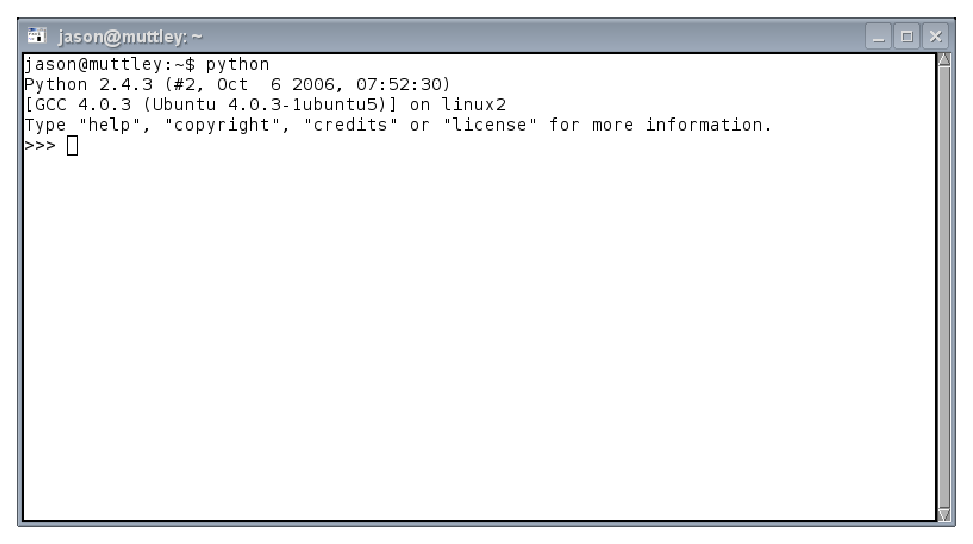
\includegraphics[width=80mm]{../en/figure4.eps}
\end{center}
\caption{Консоль Питона в Линуксе.}\label{fig4}
\end{figure}

\begin{samepage}
\note{Если ты обнаружишь, что они не прочитали инструкции в начале книги...}
\nopagebreak
\paragraph*{}
... и из-за этого у тебя не получилось что-то сделать, то перелистни эту книгу на начало, подсунь им под нос введение, пока они читают утреннюю газету, и умоляюще посмотри на них. Иногда помогает говорить «пожалуйста-пожалуйста-пожалуйста» до тех пор, пока они не встанут и не сделают всё, что надо. Ну и конечно, можно попробовать сделать всё самостоятельно, это может оказаться даже проще.
\end{samepage}

\section{Первая программа на Питоне}

Так или иначе, если ты добрался досюда, у тебя уже открыта \emph{консоль}, или командная строка Питона — это один из способов запускать команды и целые программы на Питоне. После запуска консоли или ввода любой команды ты увидишь \emph{приглашение командной строки}, которое в Питоне выглядит вот так:

\begin{verbatim}
>>>
\end{verbatim}

Если записать несколько команд на Питоне одну за другой, получится программа, которую можно запускать и не через консоль, но пока на минутку остановимся на простых командах, которые можно вводить прямиком в командную строку (после «приглашения»). Например, можно ввести туда следующую команду:

\begin{verbatim}
print("Всем привет!")
\end{verbatim}

Чтобы всё получилось, нужно ввести и скобки и кавычки (вот эти: "") так, как написано выше. Тогда на экране должно появиться что-то вроде такого:

\begin{verbatim}
>>> print("Всем привет!")
Всем привет!
\end{verbatim}

После этого приглашение командной строки появится снова, чтобы показать, что Питон готов принимать новые команды. Поздравляю! Ты только что создал и запустил свою первую программу на Питоне — пусть пока и всего из одной команды: print — функции, которая просто печатает всё, что написано в скобках. Потом мы много будет использовать эту команду.

\section{Вторая программа на питоне… опять то же самое?}

Программы на Питоне были бы не слишком полезными, если бы их приходилось каждый раз вводить заново в командную строку или если бы ты написал программу для кого-то, а ему бы пришлось её перепечатывать, чтобы запустить.

Программа для редактирования текстов (Microsoft Word, Libreoffice Writer или другая подобная), которую ты, вероятно, используешь для выполнения каких-нибудь домашних заданий, получена из исходного кода размером примерно от 10 до 100 миллионов строк. Если печатать это на бумаге с двух сторон не очень крупно, это может занять, например, 400 000 страниц. Это стопка бумаги высотой 40 метров, с десятиэтажный дом. Такое количество бумаги нести из магазина в дом, чтобы перепечатать, пришлось бы долго… очень долго…

…а если бы ещё и ветер подул в подходящий момент… за бумагой пришлось бы долго бегать. Так вот, хорошая новость: всем этим заниматься не обязательно.

\begin{center}
\includegraphics*[width=85mm]{../en/pullinghair.eps}
\end{center}

Открой текстовый редактор (можешь опять спросить у родителей, как он называется: например, kate, gedit, kdevelop, но никак не Microsoft Word, он не подойдёт) и напиши туда точно ту же самую команду, что ты до этого вводил в консоль:

\begin{verbatim}
print("Всем привет!")
\end{verbatim}

%todo save.png
Теперь сохрани этот файл в своей домашней папке. Наверху в программе должен быть значок сохранения, а когда тебя спросят, куда сохранять, нажми на какую-нибудь кнопку типа домика. В качестве имени файла введи «hello.py». Теперь опять открой терминал и напиши:

\begin{verbatim}
python hello.py
\end{verbatim}

В консоли должно появиться приветствие от программы, точно так же, как в прошлый раз (примерно как на рисунке \ref{fig9}).

\begin{figure}
\begin{center}
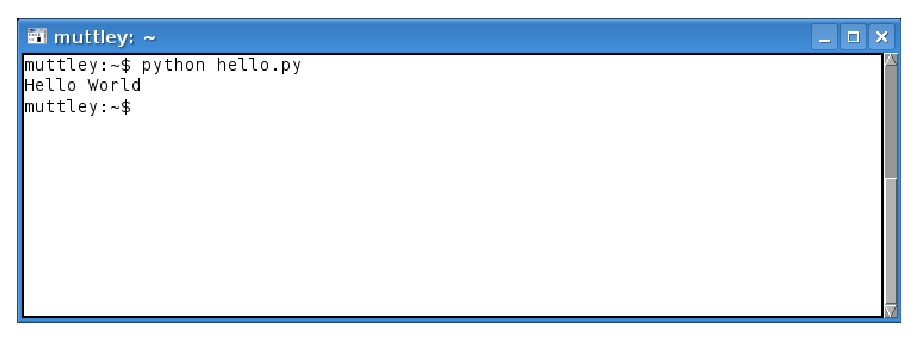
\includegraphics[width=75mm]{../en/figure9.eps}
\end{center}
\caption{Запуск программы на Питоне, сохранённой в текстовый файл}\label{fig9}
\end{figure}

Вот. Теперь ты видишь, что мудрые люди, создавшие Питон, спасли тебя от ввода одних и тех же программ много-много-много раз для выполнения одних и тех же действий. Как они делали в 1980х. Я серьёзно, им приходилось вводить каждый раз кучу команд для выполнения одной и той же программы. Можешь спросить у папы — вдруг у него был ZX81 в молодости — так там приходилось так делать. Теперь можно просто написать имя программы, и она целиком исполнится от начала до конца.

\note{Конец начала}

Добро пожаловать в удивительный мир программирования!
Мы начали с простой программы, которая печатает «Всем привет» («Hello world») — все с этого начинают, когда учатся программировать. В следующей главе мы займёмся чуть более полезными вещами в консоли Питона, а потом изучим, как написать программу посложнее.

\end{document}
